% Auto-generated by export_dashboard_networks_latex.py (nx.to_latex_raw)
% sem_yearly_2023_th0.50_mkf5 | nodes=14 edges=91
  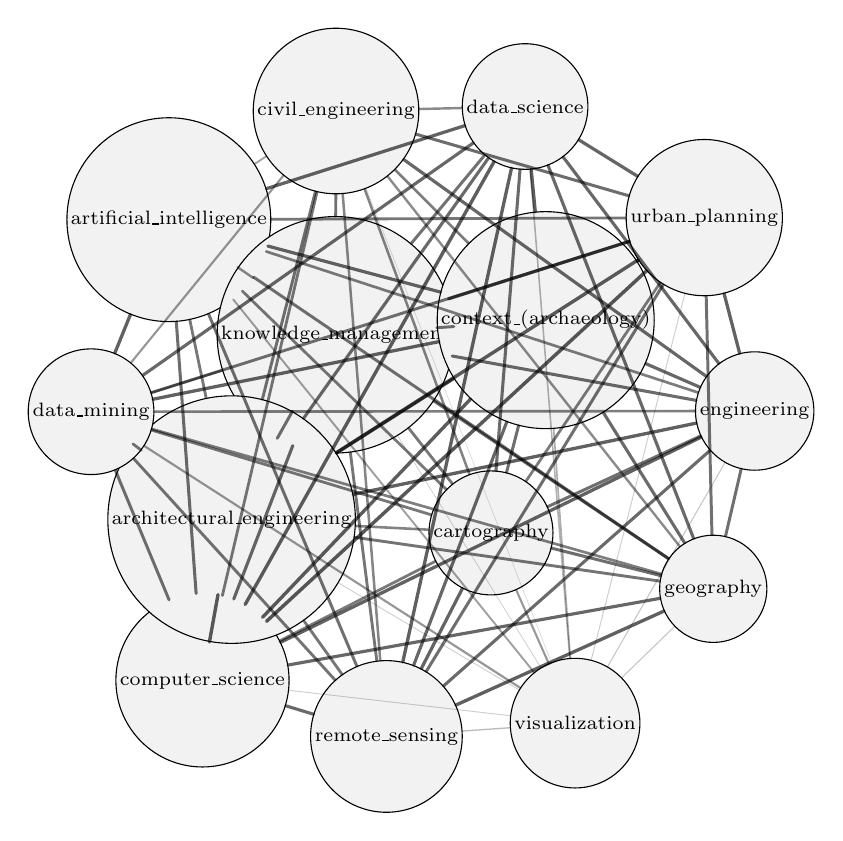
\begin{tikzpicture}[x=1cm,y=1cm,kw/.style={draw,circle,inner sep=1.2pt,font=\scriptsize,fill=black!5},concept/.style={draw,circle,inner sep=1.2pt,font=\scriptsize,fill=blue!10},method/.style={draw,rounded corners=1pt,rectangle,inner sep=1.2pt,font=\scriptsize,fill=orange!12}]
      \draw
        (1.298, 4.0) node[kw] (n0){data\_science}
        (4.214, 0.133) node[kw] (n1){engineering}
        (-2.799, -3.288) node[kw] (n2){computer\_science}
        (-3.226, 2.563) node[kw] (n3){artificial\_intelligence}
        (3.574, 2.589) node[kw] (n4){urban\_planning}
        (-1.103, 3.943) node[kw] (n5){civil\_engineering}
        (3.688, -2.125) node[kw] (n6){geography}
        (-0.463, -4.0) node[kw] (n7){remote\_sensing}
        (-1.111, 1.101) node[kw] (n8){knowledge\_management}
        (0.865, -1.415) node[kw] (n9){cartography}
        (1.933, -3.831) node[kw] (n10){visualization}
        (-2.429, -1.246) node[kw] (n11){architectural\_engineering}
        (1.56, 1.287) node[kw] (n12){context\_(archaeology)}
        (-4.214, 0.124) node[kw] (n13){data\_mining};
      \begin{scope}[-,line cap=round]
        \draw[line width=1.136pt,opacity=0.593] (n0) to (n1);
        \draw[line width=1.215pt,opacity=0.632] (n0) to (n2);
        \draw[line width=1.171pt,opacity=0.611] (n0) to (n3);
        \draw[line width=1.156pt,opacity=0.603] (n0) to (n4);
        \draw[line width=0.875pt,opacity=0.462] (n0) to (n5);
        \draw[line width=1.131pt,opacity=0.590] (n0) to (n6);
        \draw[line width=1.199pt,opacity=0.625] (n0) to (n7);
        \draw[line width=1.064pt,opacity=0.557] (n0) to (n8);
        \draw[line width=1.109pt,opacity=0.580] (n0) to (n9);
        \draw[line width=0.562pt,opacity=0.306] (n0) to (n10);
        \draw[line width=1.123pt,opacity=0.586] (n0) to (n11);
        \draw[line width=1.214pt,opacity=0.632] (n0) to (n12);
        \draw[line width=1.137pt,opacity=0.594] (n0) to (n13);
        \draw[line width=1.181pt,opacity=0.615] (n1) to (n2);
        \draw[line width=0.971pt,opacity=0.511] (n1) to (n3);
        \draw[line width=1.182pt,opacity=0.616] (n1) to (n4);
        \draw[line width=1.143pt,opacity=0.597] (n1) to (n5);
        \draw[line width=1.078pt,opacity=0.564] (n1) to (n6);
        \draw[line width=1.121pt,opacity=0.586] (n1) to (n7);
        \draw[line width=1.108pt,opacity=0.579] (n1) to (n8);
        \draw[line width=1.080pt,opacity=0.565] (n1) to (n9);
        \draw[line width=0.386pt,opacity=0.218] (n1) to (n10);
        \draw[line width=1.197pt,opacity=0.624] (n1) to (n11);
        \draw[line width=1.141pt,opacity=0.596] (n1) to (n12);
        \draw[line width=0.962pt,opacity=0.506] (n1) to (n13);
        \draw[line width=1.099pt,opacity=0.574] (n2) to (n3);
        \draw[line width=1.250pt,opacity=0.650] (n2) to (n4);
        \draw[line width=1.007pt,opacity=0.529] (n2) to (n5);
        \draw[line width=1.143pt,opacity=0.596] (n2) to (n6);
        \draw[line width=1.126pt,opacity=0.588] (n2) to (n7);
        \draw[line width=1.129pt,opacity=0.589] (n2) to (n8);
        \draw[line width=0.998pt,opacity=0.524] (n2) to (n9);
        \draw[line width=0.339pt,opacity=0.194] (n2) to (n10);
        \draw[line width=1.231pt,opacity=0.641] (n2) to (n11);
        \draw[line width=1.223pt,opacity=0.637] (n2) to (n12);
        \draw[line width=1.066pt,opacity=0.558] (n2) to (n13);
        \draw[line width=1.024pt,opacity=0.537] (n3) to (n4);
        \draw[line width=0.672pt,opacity=0.361] (n3) to (n5);
        \draw[line width=1.057pt,opacity=0.553] (n3) to (n6);
        \draw[line width=1.074pt,opacity=0.562] (n3) to (n7);
        \draw[line width=0.860pt,opacity=0.455] (n3) to (n8);
        \draw[line width=1.003pt,opacity=0.526] (n3) to (n9);
        \draw[line width=0.691pt,opacity=0.371] (n3) to (n10);
        \draw[line width=1.015pt,opacity=0.533] (n3) to (n11);
        \draw[line width=1.157pt,opacity=0.603] (n3) to (n12);
        \draw[line width=1.192pt,opacity=0.621] (n3) to (n13);
        \draw[line width=1.091pt,opacity=0.571] (n4) to (n5);
        \draw[line width=1.073pt,opacity=0.561] (n4) to (n6);
        \draw[line width=1.076pt,opacity=0.563] (n4) to (n7);
        \draw[line width=1.159pt,opacity=0.604] (n4) to (n8);
        \draw[line width=0.987pt,opacity=0.518] (n4) to (n9);
        \draw[line width=0.341pt,opacity=0.195] (n4) to (n10);
        \draw[line width=1.223pt,opacity=0.637] (n4) to (n11);
        \draw[line width=1.236pt,opacity=0.643] (n4) to (n12);
        \draw[line width=1.053pt,opacity=0.552] (n4) to (n13);
        \draw[line width=0.861pt,opacity=0.455] (n5) to (n6);
        \draw[line width=0.904pt,opacity=0.477] (n5) to (n7);
        \draw[line width=1.070pt,opacity=0.560] (n5) to (n8);
        \draw[line width=0.913pt,opacity=0.481] (n5) to (n9);
        \draw[line width=0.250pt,opacity=0.150] (n5) to (n10);
        \draw[line width=1.053pt,opacity=0.551] (n5) to (n11);
        \draw[line width=0.967pt,opacity=0.508] (n5) to (n12);
        \draw[line width=0.768pt,opacity=0.409] (n5) to (n13);
        \draw[line width=1.198pt,opacity=0.624] (n6) to (n7);
        \draw[line width=1.059pt,opacity=0.555] (n6) to (n8);
        \draw[line width=1.085pt,opacity=0.567] (n6) to (n9);
        \draw[line width=0.398pt,opacity=0.224] (n6) to (n10);
        \draw[line width=1.040pt,opacity=0.545] (n6) to (n11);
        \draw[line width=1.115pt,opacity=0.583] (n6) to (n12);
        \draw[line width=0.962pt,opacity=0.506] (n6) to (n13);
        \draw[line width=1.032pt,opacity=0.541] (n7) to (n8);
        \draw[line width=1.166pt,opacity=0.608] (n7) to (n9);
        \draw[line width=0.484pt,opacity=0.267] (n7) to (n10);
        \draw[line width=1.026pt,opacity=0.538] (n7) to (n11);
        \draw[line width=1.142pt,opacity=0.596] (n7) to (n12);
        \draw[line width=1.040pt,opacity=0.545] (n7) to (n13);
        \draw[line width=1.019pt,opacity=0.535] (n8) to (n9);
        \draw[line width=0.306pt,opacity=0.178] (n8) to (n10);
        \draw[line width=1.071pt,opacity=0.561] (n8) to (n11);
        \draw[line width=1.061pt,opacity=0.555] (n8) to (n12);
        \draw[line width=0.819pt,opacity=0.435] (n8) to (n13);
        \draw[line width=0.758pt,opacity=0.404] (n9) to (n10);
        \draw[line width=0.934pt,opacity=0.492] (n9) to (n11);
        \draw[line width=1.088pt,opacity=0.569] (n9) to (n12);
        \draw[line width=1.008pt,opacity=0.529] (n9) to (n13);
        \draw[line width=0.328pt,opacity=0.189] (n10) to (n11);
        \draw[line width=0.593pt,opacity=0.322] (n10) to (n12);
        \draw[line width=0.776pt,opacity=0.413] (n10) to (n13);
        \draw[line width=1.179pt,opacity=0.615] (n11) to (n12);
        \draw[line width=1.016pt,opacity=0.533] (n11) to (n13);
        \draw[line width=1.187pt,opacity=0.619] (n12) to (n13);
      \end{scope}
    \end{tikzpicture}
